\documentclass[12pt]{article}

\usepackage{setspace}
\usepackage{natbib}
\usepackage{graphicx}
\usepackage{fancyheadings}
\usepackage{amsmath}
\usepackage{url}
\usepackage[top=1.25in, bottom=1.25in, left=1.25in, right=1.25in]{geometry}
\usepackage[short]{datetime}
\usepackage{lipsum}

\doublespacing

\usepackage{authblk}
\renewcommand\Affilfont{\small}

\title{This is the title of the manuscript}

\author[1,2,3,*]{Paul L. Gribble}
\author[1,2,4]{Jeremy Wong}

\affil[1]{Centre for Brain and Mind, The University of Western Ontario}
\affil[2]{Department of Psychology, The University of Western Ontario}
\affil[3]{Department of Physiology \& Pharmacology, Schulich School of Medicine \& Dentistry}
\affil[4]{Graduate Program in Neuroscience, The University of Western Ontario}

\date{}

\begin{document}

\begin{singlespace}

\maketitle
\thispagestyle{empty}

\hfill

\begin{flushleft}

\textbf{Mailing Address:}\\
\vspace{2ex}
Professor Paul Gribble\\
Centre for Brain and Mind\\
Department of Psychology\\
The University of Western Ontario\\
1151 Richmond St\\
London, Ontario\\
Canada N6A 5B7\\
\vspace{1em}
Phone: +1 519.661.2111 ext. 86185\\
Fax: +1 519.661.3613\\
email: \url{paul@gribblelab.org}

\vspace{2em}
$^{*}$ Corresponding author email: \url{paul@gribblelab.org}

\vspace{3em}
\textbf{Keywords}: blah; blah blah; blah blah blah

\vfill
\textbf{Manuscript version}: \today, \currenttime

\end{flushleft}

\end{singlespace}

\newpage
\section*{Abstract}

\lipsum[1]

\newpage
\section*{Introduction}

Blah blah blah lots of crazy research has been done on this topic \citep{Mattar:2005}. \lipsum[1]

\lipsum[1-3]

\section*{Methods}

\lipsum[1-3]

\section*{Results}

\lipsum[1-3]

\section*{Discussion}

\lipsum[1-3]

\newpage
\section*{Acknowledgements}
This research was supported by grants to PLG by the Canadian Institutes of Health Research and the Natural Sciences and Engineering Council of Canada.

\newpage
\bibliographystyle{jneurosci} 
\bibliography{articletemplaterefs}

\newpage
\subsection*{Figure Titles}
\begin{flushleft}

\vspace{.5cm}
{\bf Figure~\ref{fig:setupfig}.} Blah blah blah the robot setup blah.

\end{flushleft}

\newpage
\clearpage
\begin{figure}[H]
	\centering
    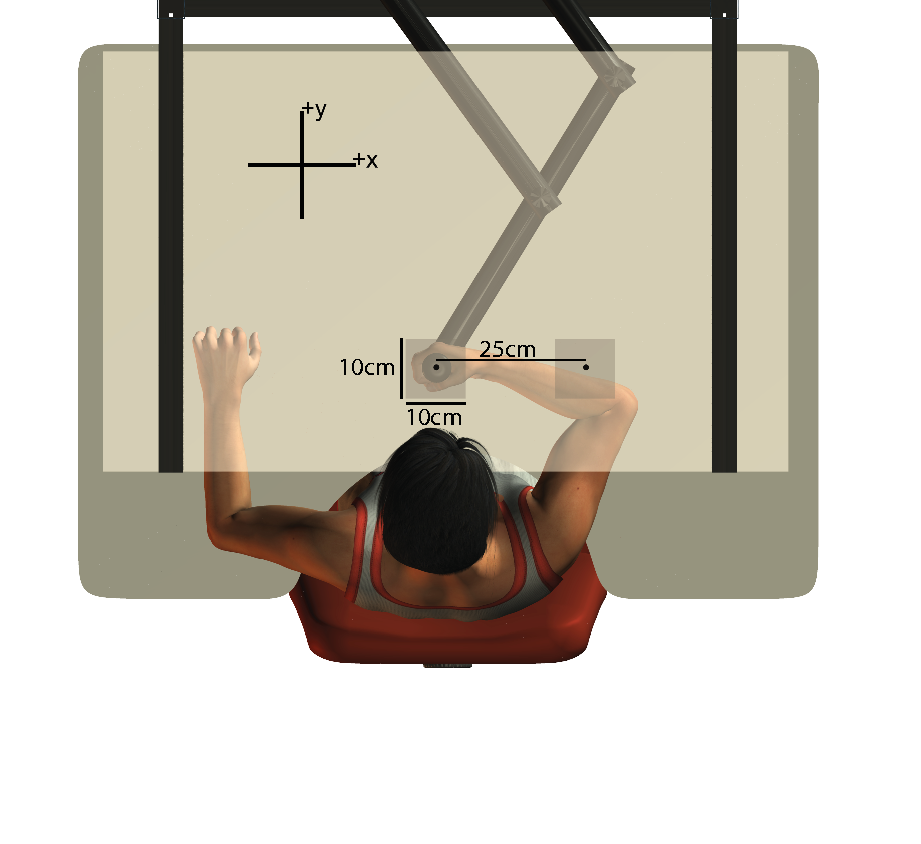
\includegraphics[height=3in]{articletemplatefigure.pdf}
 \caption{}
 \label{fig:setupfig}
\end{figure}

\end{document}

